\documentclass{article}

\usepackage[margin=2.5cm]{geometry}

\usepackage[T1]{fontenc} 
\usepackage{mathpazo}
%\usepackage{newcent}
%\usepackage{fbb}
%\usepackage{fourier}

\usepackage[utf8]{inputenc}
\usepackage{amsfonts} 
\usepackage{array} 
\usepackage{enumitem}
\usepackage{tabularx}
\usepackage{graphicx}
\usepackage{fancyhdr}
\usepackage{fancyvrb}
\usepackage{amsmath}
\usepackage{amsthm}
\usepackage[most]{tcolorbox}
\tcbuselibrary{breakable}
\usepackage{float}
\usepackage{listings}  
\usepackage{xcolor}
\usepackage{subfigure}
\usepackage[htt]{hyphenat}
\usepackage{hyperref}
\usepackage{verbatim}

%%%%%%%%%%%%%%%%%%%%% BIB %%%%%%%%%%%%%%%%%%%%%%%%%%%%%%%
\usepackage[backend=biber,style=apa,autocite=inline]{biblatex}
\DeclareLanguageMapping{english}{english-apa}
\addbibresource{mem.bib}
%%%%%%%%%%%%%%%%%%%%%%%%%%%%%%%%%%%%%%%%%%%%%%%%%%%%%%%%%

\definecolor{codegreen}{rgb}{.2,0.6,0}
\definecolor{codegray}{rgb}{0.5,0.5,0.5}
\definecolor{codepurple}{rgb}{0.58,0,0.82}
\definecolor{codeblue}{rgb}{0,0.4,0.82}
\definecolor{codeorange}{rgb}{0.94,0.34,0.0}
\definecolor{backcolour}{rgb}{0.95,0.95,0.92}
\definecolor{backcolourgray}{rgb}{0.92,0.92,0.92}
\definecolor{codewhite}{rgb}{1,1,1}

\lstdefinestyle{mystyle}{
    backgroundcolor=\color{backcolourgray},   
    commentstyle=\color{codegreen},
    keywordstyle=\color{codeblue},
    numberstyle=\tiny\color{black},
    stringstyle=\color{codeorange},
    basicstyle=\ttfamily\footnotesize,
    breakatwhitespace=false,         
    breaklines=true,                 
    captionpos=b,                    
    keepspaces=true,                 
    %numbers=left,                    
    numbersep=5pt,                  
    showspaces=false,                
    showstringspaces=false,
    showtabs=false,                  
    tabsize=2,
    extendedchars=true,
    frame=single
    %, basicstyle=\footnotesize
}
\lstset{style=mystyle}

\usepackage{hyperref}
\hypersetup{
    colorlinks=true,
    allcolors=blue,
    %linkcolor=green,
    %filecolor=magenta,      
    %urlcolor=blue,
    %citecolor=blue,
}

\pagestyle{fancy}
\fancyhf{}
\rhead{AI. Practice 3.}
\lhead{Pablo Cuesta Sierra, Álvaro Zamanillo Sáez - G2351, P05}
\cfoot{\thepage}

\usepackage[toc,title]{appendix}

\usepackage{titlesec}
%\titleformat*{\subsection}{\large\bfseries\color{darkgray}}
%\titleformat*{\subsubsection}{\normalsize\itshape\color{darkgray}}

%\setlength{\parskip}{0.15cm}


%parameters: file, caption, label, scale
\newcommand{\myFigure}[4]{%
    \begin{figure}[H]
        \includegraphics[width=#4\textwidth]{#1}
        \centering
        \caption{#2}
        \label{#3}
    \end{figure}
}

%grey item for enumerate
%\renewcommand{\thesubsubsection}{(\thesubsection.\alph{subsubsection})}
\setcounter{secnumdepth}{4}
\setcounter{tocdepth}{3}
%\newcommand{\question}[1]{\subsection{#1}}
%\newcommand{\subquestion}[1]{\subsubsection{#1}}


\setcounter{section}{0}


\title{\textbf{Artificial Intelligence. Practice 3.}}
\author{\textbf{Pablo Cuesta Sierra, Álvaro Zamanillo Sáez} \\Group 2351. Pair 5.}
%\date{}

\begin{document}

%\vspace*{-1.5cm}
{
    %\let\newpage\relax
    \maketitle
}

%\begin{tcolorbox}
\tableofcontents
%\end{tcolorbox}

\newpage
\section{Reading exercise.}

The predicate \texttt{slice/4} extracts a slice from a list, between two given indices of that list. The code is the following:

\lstinputlisting[language=prolog, captionpos=t, caption={\emph{slice/4}}]{files/slice.pl}

\subsection{Declarative reading.}

The previous definition of \texttt{slice/4} has 3 clauses. We will now read the definition declaratively:

\begin{enumerate}
    \item The slice of a list $L$ between indices 1 and 1 is the list containing only the first element of $L$.
    \item If \texttt{K>1} and \texttt{Ys} is the slice of \texttt{Xs} between 1 and \texttt{K-1}, then \texttt{[X|Ys]} is the slice of \texttt{[X|Xs]} between 1 and \texttt{K}.
    \item If \texttt{I>1} and \texttt{Ys} is the slice of \texttt{Xs} between \texttt{I-1} and \texttt{K-1}, then \texttt{Ys} is the slice of \texttt{[\_|Xs]} between \texttt{I} and \texttt{K}.
\end{enumerate}

\subsection{Procedural reading.}

Query: \texttt{slice([1, 2, 3, 4], 2, 3, L2).}

\begin{enumerate}
    \item Does the first clause apply? No: 2 does not unify with 1.
    \item Does the second clause apply? No: 2 does not unify with 1.
    \item Does the third clause apply? Yes: \texttt{Xs:=[2,3,4]}, \texttt{I:=2}, \texttt{K:=3}, \texttt{Ys:=L2}. 
    \item The three first goals are: \texttt{I>1} (true), \texttt{I1} unifies with 1 and \texttt{K1} unifies with 2. 
    \item Now, the goal: \texttt{slice(Xs, I1, K1, Ys)}, in this case: \texttt{slice([2,3,4], 1, 2, L2)}.
    \begin{enumerate}
        \item Does the first clause apply? No: 2 does not unify with 1. 
        \item Does the second clause apply? Yes: \texttt{X':=2}, \texttt{Xs':=[3,4]}, \texttt{K':=2}, \texttt{[2|Ys']:=L2}.
        \item The two first goals are: \texttt{K'>1} (true), \texttt{K1'} unifies with 1. 
        \item Now, the goal: \texttt{slice(Xs', 1, K1', Ys')}, in this case: \texttt{slice([3,4], 1, Ys')}.
        \begin{enumerate}
            \item Does the first clause apply? Yes: \texttt{X'':=3}, \texttt{[X'']:=[3]}.
        \end{enumerate}
        \item The previous goal exits with \texttt{Ys'=[3]}
    \end{enumerate}
    \item The previous goal exits with \texttt{L2=[2|Ys']=[2,3]}
\end{enumerate}
Finally the query exits with \texttt{L2=[2,3]}.


\newpage
\setcounter{section}{8}
\section{K nearest neighbours.}

\setcounter{subsection}{4}
\subsection{Application to a real database.}

The nearest neighbours algorithm predicts the class to which a specfic instance belongs given a collection of training data. The $K$ refers to the number of elements around the instance (the metric used in this case is the euclidean distance) that are going to be considered to determine its class.

If $K=1$, the class assigned to our instance is the one from the closest neighbour. As we increase $K$, the class assigned is the most frequent from the K closest neighbours. Having said this, it is clear that the performance of the algorithm does not only depend on the training data given but also in the value that $K$ takes. The optimal value of $K$ depends on the size of the training data and its accuracy. 

In the last line of the next image, it is observed that the size of our training data is 150. In general, larger sets of training data make the optimal value of $K$ smaller. This is due to the fact that it is likely to happen that for any point we want to classify, it exists another in the training set which is actually really close to it, and therefore, they can be considered of the same class with a low probability of error.

\myFigure{./img/trace2.png}{Partial trace of the K nearest neighbours algorithm. The length of our data is 150.}{trace}{.9}

Firstly, we will comment the effect of $K$ being too large. In our case, selections of $K$ near to 150 would obviously be useless as we would be considering almost every point of the data set as a ``near'' neighbour. Thus, the distinction to assign a class would be the frequency of the training set rather than the distance of our point to the rest.

On the other hand, extremely small values of $K$ may be susceptible to noise and are too dependant to the training data. As commented before, if the training set is large enough, this may not be a real problem. 

\myFigure{./img/hitRate.png}{Hit rate varying K.}{hitRate}{.65}

As seen in figure \ref{hitRate}, the maximum hit rate (0.98) in our case is obtained with values of $K\in\{19,21\}$. It is worth mentioning that the performance of the algorithm for small values of $K$ ($K\in\{1,2,...,20\}$) does not differ considerably from the maximum hit rate. Indeed the difference is about just a $2\%$. This small difference can be explained with the size of the training set; once again, larger training sets make the optimal value of $K$ smaller. 

Finally, if we analyze the rest of values (figure \ref{graph}), we observe that after the values that maximize the hit rate, the performance of the algorithm decreases and once $K$ reaches $2/3$ of the size of the training data, the hit rate is below the $52\%$. This makes sense, as there are exactly 50 samples of each of the 3 classes. Therefore, when taking $K \geq 100$, we will be considering, at most, only $49$ samples of the correct class, which is less than a halve of $K$. This explains the drastic drop of the hit rate.


\myFigure{./img/gnuplot_graph.png}{Graph of the hit rate with respect to $K$.}{graph}{.8}

One would expect that, if there is a higher proportion of a class $C_1$ within the training data, using $K$ close to the number of samples (150 in this case) would make the hit rate close to the proportion of said class $C_1$. However, the classes are equally represented in our data (3 classes with 50 samples); therefore, when we take one out in order to make a prediction, for $K$ close to 150, the prediction fails and the hit rate drops to~0.

\newpage
\section{Creation of fractals.}

The idea of the fractal proposed in the assignment is the following:

\begin{enumerate}
    \item Depth 0 paints a line between two given points.
    \item Depth $d>0$ takes two points ($P$ and $Q$) and paints four fractals of depth $d-1$ between points $P$ and $R$, $R$ and $S$, $S$ and $T$, $T$ and $Q$; where points $R$, $S$, $T$ are points defined relative to $P$ and $Q$: 
\end{enumerate}

\myFigure{./files/fractal}{Visual representation of the relative positions of the points.}{img:fractal}{.6}

If points are seen as vectors, with respect to any origin, the definitions are the following (note that $P$ and $Q$ are given):

\[
    \text{Dif} = \frac{Q-P}{3}
\] 
\[
    \text{Dif\_ort} = \textbf{R}_{\pi/2}(\text{Dif})
\]
\[
    R = P + \text{Dif}
\]
\[
    T = R + \text{Dif}
\]
\[
    S = R + \cos\left(\frac{\pi}{3}\right)\text{Dif} + \sin\left(\frac{\pi}{3}\right)\text{Dif\_ort} = R + \frac{\text{Dif} + \sqrt{3}\text{Dif\_ort}}{2}.
\]

Note: $\textbf{R}_{\pi/2}(v)$ denotes the rotation of a vector $v\in\mathbb{R}^{2}$ of $\pi/2$ radians with respect to the origin. 

Therefore, the base case (depth 0) displays a single line; whereas the general case: depth $d$ calculates the $R$, $S$, $T$ points with the given $P$ and $Q$, and calls the recursive function with depth $d-1$ on the four lines that were before explained.

\vspace{.5cm}
Pictures of our fractals:

\myFigure{./img/d0}{Depth 0.}{d}{.6}
\myFigure{./img/d1}{Depth 1.}{d}{.6}
\myFigure{./img/d2}{Depth 2.}{d}{.6}
\myFigure{./img/d3}{Depth 3.}{d}{.6}
\myFigure{./img/d4}{Depth 4.}{d}{.6}


\newpage
\begin{appendices}
\section{Alternative codification.}
\subsubsection*{Computation of the most relevant labels (9.3.1), another implementation.}

In this exercise, we had to implement the predicate \texttt{calcular\_K\_etiquetas\_mas\_relevantes(Y\_entrenamiento, K, Vec\_distancias, K\_etiquetas)}.

The implementation that we included in the code file makes use of the data structure `Pairs', from prolog; with built-in predicates. The idea is to sort the tags from \texttt{Y\_entrenamiento} by the distances in \texttt{Vec\_distancias} and select the \texttt{K} first ones. 

Another option, to implement the same idea, would be to manually code the sort predicate:

\begin{lstlisting}[language=prolog, captionpos=t, caption={Alternate implementation of \texttt{calcular\_K\_etiquetas\_mas\_relevantes/4}.}]
/***************
* EJERCICIO 9e. calcular_K_etiquetas_mas_relevantes/4
*
*       ENTRADA:
*               Y_entrenamiento: Vector de valores alfanumericos de una distribucion categorica. Cada etiqueta corresponde a una instancia de X_entrenamiento.
*               K: Numero de valor entero.
*               Vec_distancias: Vector de valores reales correspondiente a una fila de Matriz_resultados.
*       SALIDA:
*		K_etiquetas: Vector de valores alfanumericos de una distribucion categorica.
*
****************/
calcular_K_etiquetas_mas_relevantes(Y_Entrenamiento, K, Distancias, Etiquetas):-
    create_tuples(Y_Entrenamiento,Distancias,Tuples),
    sort_tuples(Tuples,SortedTuples),
    first_K_tags(K,SortedTuples,Etiquetas).


/**
* Extract the first K tags of a list of tuples [Tag,Value]
* Input: List of tuples
* Output: List of K tags
*/
first_K_tags(0,_,[]):-!.
first_K_tags(K,[[Tag,_]|SortedTuples],[Tag|Etq]):-
    Ks is K-1,
    first_K_tags(Ks,SortedTuples,Etq).
    
/**
* create_tuples(Y_Entrenamiento,Distancias,Tuples)
* Creates list of tuples [tag,distance]
* Input: List of tags (['a','b','a']) list of distances ([1,5,4])
* Output: list of tuples ([['a',1],['b',5],['a',4]])
*/
create_tuples([],[],[]):-!.
create_tuples([E|Es],[D|Ds],Tuples):-
    create_tuples(Es,Ds,Rs),
    Tuples=[[E,D]|Rs].

/**
* sort_tuples(UnsortedList, SortedList).
* Sorts a list of elements of type [TAG,DISTANCE]
* Input: unsorted list
* Output: sorted list
*/
sort_tuples([],[]):-!.
sort_tuples([X|Xs],Sorted):-
    sort_tuples(Xs,Xs_Sorted),
    insert_in_order(X,Xs_Sorted,Sorted).

/**
* insert_in_order([TAG,DISTANCE],List,NewSortedList)
* Inserts an element of type [tag,distance ]in a sorted list by distance
* Input: element to insert and sorted list
* Output: New sorted list that contains the element given as input
*/
insert_in_order([Tag,K],[],[[Tag,K]]):-!.
insert_in_order([Tag,K],[[T,N]|Tail],[[Tag,K]|[[T,N]|Tail]]):- K<N,!.
insert_in_order([Tag,K],[[T,N]|Tail],[[T,N]|Xs]):-
    insert_in_order([Tag,K],Tail,Xs).
\end{lstlisting} 


\end{appendices}


\end{document}


%% ejemplos :
\begin{lstlisting}[language=python, caption = The Node class (\emph{search.py}),captionpos=t]
\end{lstlisting}


\myFigure{./img/ex6/test6}{Results of the autograder tests}{test6}{.9}




\begin{figure}[H]
    \centering
    \begin{subfigure}
        %\caption{Code}
        %\label{code.1}
        \begin{lstlisting}
            weights = [
              [100,-10, 11,  6,  6, 11,-10,100],
              [-10,-20,  1,  2,  2,  1,-20,-10],
              [ 10,  1,  5,  4,  4,  5,  1, 10],
              [  6,  2,  4,  2,  2,  4,  2,  6],
              [  6,  2,  4,  2,  2,  4,  2,  6],
              [ 10,  1,  5,  4,  4,  5,  1, 10],
              [-10,-20,  1,  2,  2,  1,-20,-10],
              [100,-10, 11,  6,  6, 11,-10,100],
            ]
                    \end{lstlisting}
    \end{subfigure}
    %\subfigure[]{} 
    %\subfigure[]{}
    \caption{Weighted boards.}
    \centering
    \label{weighted_boards213231}
\end{figure}

\begin{figure}[H]
    \centering
    \subfigure[]{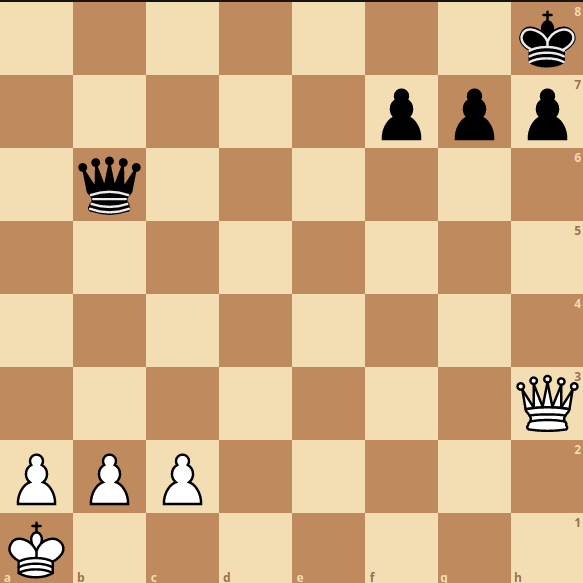
\includegraphics[width=.8\textwidth]{./images/tablero1.png}} 
    \subfigure[]{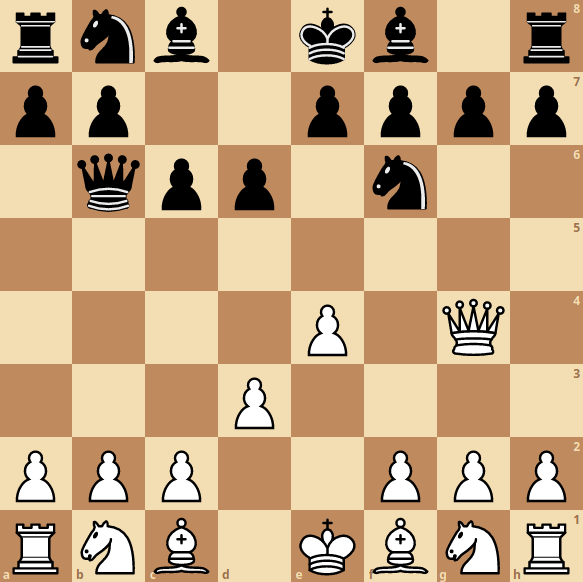
\includegraphics[height=0.45\textwidth]{./images/tablero2.png} 
    \caption{Execution of the eightpuzzle}
    \centering
    \label{8p}
\end{figure}